% ==========================================================================
% ogclews-link -- a technical introduction.
% Intro -> overview -> channels -> channels in detail -> software -> MUIOGO.
% Reuses the five self-titled figures in coupling-diagrams/*.pdf and the shared
% editorial palette (theme/ogclews-colors). Build: latexmk -pdf ogclews-link.tex
% ==========================================================================
\documentclass[aspectratio=169,11pt]{beamer}

\usepackage[T1]{fontenc}
\usepackage[scaled=1.0]{helvet}            % editorial sans (body)
\usepackage[scaled=1.03]{XCharter}         % transitional serif (titles) -- matches the figures
\renewcommand{\familydefault}{\sfdefault}  % sans stays default; serif via \rmfamily
\usefonttheme{professionalfonts}
\usepackage{microtype}
\hyphenpenalty=10000 \exhyphenpenalty=10000 \emergencystretch=2em \hbadness=10000  % no mid-word breaks
\usepackage{amsmath,amssymb}
\usepackage{graphicx}
\usepackage{booktabs}
\usepackage{array}
\usepackage{tikz}
\usetikzlibrary{arrows.meta}

% OG-Core x CLEWS — shared color palette.
% Single source of truth, mirrored from ogclews_link/style.py (the matplotlib figure
% theme) so the TikZ diagrams, the Beamer deck, and the data figures all share one
% editorial, colorblind-safe palette. \input this from any preamble; it only defines
% colors (no package loads), so it is safe in both standalone and beamer documents.

\definecolor{ink}{HTML}{222222}      % primary text / heavy rules
\definecolor{sub}{HTML}{555555}      % secondary text
\definecolor{mute}{HTML}{888888}     % tertiary / source lines
\definecolor{grid}{HTML}{E6E6E6}     % faint rules, fills

% the two models + policy — the load-bearing semantic colors
\definecolor{ogc}{HTML}{0F5499}      % OG-Core      (FT oxford blue)
\definecolor{clews}{HTML}{0D7680}    % CLEWS/OSeMOSYS (teal)
\definecolor{policy}{HTML}{E3120B}   % policy lever (Economist red)

% accents / signed values (match style.py)
\definecolor{claret}{HTML}{990F3D}   % kicker rule
\definecolor{gain}{HTML}{2166AC}     % positive change (blue)
\definecolor{loss}{HTML}{B2182B}     % negative change (red)
\definecolor{amber}{HTML}{E69F00}    % categorical 4
\definecolor{purple}{HTML}{7A6FAC}   % categorical 5
\definecolor{slate}{HTML}{7F8C8D}    % categorical 6 / neutral

% sequential blue ramp (ordered income groups, poorest -> richest)
\definecolor{seqA}{HTML}{C6DBEF}
\definecolor{seqB}{HTML}{9ECAE1}
\definecolor{seqC}{HTML}{6BAED6}
\definecolor{seqD}{HTML}{4292C6}
\definecolor{seqE}{HTML}{2171B5}
\definecolor{seqF}{HTML}{08519C}
\definecolor{seqG}{HTML}{08306B}

\definecolor{paper}{HTML}{FBF7F0}          % warm canvas (matches the figures)

% ---- editorial beamer theme keyed to the figure palette ---------------------
\setbeamertemplate{navigation symbols}{}
\setbeamercolor{background canvas}{bg=paper}
\setbeamercolor{normal text}{fg=ink}
\setbeamercolor{frametitle}{fg=ink}
\setbeamercolor{structure}{fg=ogc}
\setbeamercolor{itemize item}{fg=claret}
\setbeamercolor{itemize subitem}{fg=clews}
\setbeamercolor{block title}{fg=white,bg=ogc}
\setbeamercolor{block body}{fg=ink,bg=ogc!6}
\setbeamerfont{frametitle}{series=\bfseries}
\setbeamertemplate{itemize item}{\small\raise0.6pt\hbox{\textbullet}}
\setbeamertemplate{itemize subitem}{\footnotesize\raise0.6pt\hbox{--}}

% frametitle: claret kicker rule + serif bold ink title (mirrors the figures' header)
\setbeamertemplate{frametitle}{%
  \vspace{0.5cm}%
  {\color{claret}\rule{0.62cm}{2.2pt}}\par\vspace{3pt}%
  {\rmfamily\bfseries\Large\color{ink}\insertframetitle}\par\vspace{1pt}}

\setbeamertemplate{footline}{%
  \hbox to\paperwidth{\hspace{0.5cm}%
    {\color{mute}\scriptsize \texttt{ogclews-link}\, $\cdot$\, OG-Core $\times$ CLEWS}%
    \hfill{\color{mute}\scriptsize\insertframenumber\,/\,\inserttotalframenumber}%
    \hspace{0.5cm}}\vspace{3pt}}

\newcommand{\kick}[1]{{\scriptsize\bfseries\color{claret}\MakeUppercase{#1}}}
\newcommand{\code}[1]{{\ttfamily\small #1}}

% full-bleed, self-titled figure frame (the figure carries its own header)
\newcommand{\figframe}[2]{%
  \begin{frame}[plain]\centering\vfill
    \includegraphics[width=0.97\linewidth,height=0.84\textheight,keepaspectratio]{coupling-diagrams/#1.pdf}\par
    \vspace{3pt}{\scriptsize\color{mute}#2}\vfill\end{frame}}

% editorial section divider
\newcommand{\sectiondiv}[2]{%
  \begin{frame}[plain]\vfill\hspace{0.7cm}\begin{minipage}{0.86\paperwidth}
    {\color{claret}\rule{1.0cm}{2.5pt}}\par\vspace{9pt}
    \kick{#1}\par\vspace{5pt}
    {\rmfamily\bfseries\huge\color{ink}#2}\par
  \end{minipage}\vfill\end{frame}}

\begin{document}

% ============================ TITLE =======================================
\begin{frame}[plain]
  \vfill\hspace{0.7cm}\begin{minipage}{0.86\paperwidth}
  {\color{claret}\rule{1.3cm}{2.6pt}}\par\vspace{12pt}
  {\rmfamily\bfseries\LARGE\color{ink}\texttt{ogclews-link}}\par\vspace{6pt}
  {\rmfamily\Large\color{ink}A soft link between a macroeconomy and an energy system}\par\vspace{12pt}
  {\large\color{sub}OG-Core $\times$ CLEWS/OSeMOSYS --- passing prices, quantities and\\ emissions between the two, channel by channel}\par\vspace{20pt}
  {\footnotesize\color{mute}OG-PHL calibration\, $\cdot$\, \texttt{ogclews-link}\, $\cdot$\, \today}\par
  \end{minipage}\vfill
\end{frame}

% ============================ 1. INTRODUCTION =============================
\sectiondiv{Introduction}{What the link is, and why}

\begin{frame}{Two analyses that don't usually meet}
  Energy-transition pathways and their economic consequences are normally studied with
  \textbf{separate models that don't share inputs}.
  \medskip
  \begin{itemize}\setlength\itemsep{8pt}
    \item A least-cost \textbf{energy} model (CLEWS / OSeMOSYS) gives the build-out, electricity
          prices and emissions --- but is blind to wages, the public budget, household welfare,
          and who gains or loses.
    \item A \textbf{macroeconomic} model (OG-Core) gives those --- households by age and income,
          industries, the fiscal sector --- but treats energy as a bare price and quantity, with
          no representation of the system that supplies it.
  \end{itemize}
  \medskip
  {\color{ink}\texttt{ogclews-link} couples the two}: a change on the energy side carries through to
  the economy, and the economy's response carries back.
\end{frame}

\begin{frame}{\texttt{ogclews-link} in one slide}
  \begin{itemize}\setlength\itemsep{8pt}
    \item A \textbf{soft link}: the two models stay separate and pass a few numbers between them ---
          they solve in incompatible ways, so they can't be merged into one.
    \item Each crossing is a named \textbf{channel} --- a checked recipe that turns something CLEWS
          produces into a parameter OG-Core understands.
    \item \textbf{Country-agnostic}: nothing about the country is hard-coded --- the industries (and
          which one is electricity) are read from the calibration and worked out for each run.
    \item \textbf{Auditable}: every channel records what it changed, and built-in checks stop the same
          effect being counted twice.
  \end{itemize}
  \vfill
  {\footnotesize\color{sub}The key number passed is the energy system's \emph{marginal} cost of electricity
  --- what the next unit actually costs to supply --- not an assumed or averaged price.}
\end{frame}

% ============================ 2. OVERVIEW ================================
\sectiondiv{Overview}{The two models, joined channel by channel}

\figframe{system-map}{Both models bookend three direction-grouped bands; each line names the channel and,
in small type, its function in the code.}

\begin{frame}{The seam: numbers out, parameters in}
  \begin{columns}[T]
    \begin{column}{0.5\textwidth}
      \textbf{\color{clews}From CLEWS --- what it sends}\\[4pt]
      {\small read from a solved energy scenario:}
      \begin{itemize}\setlength\itemsep{4pt}\small
        \item the \textbf{marginal cost of electricity} (what the next unit costs to supply)
        \item the capital a build-out requires
        \item emissions (PM2.5, CO$_2$)
      \end{itemize}
    \end{column}
    \begin{column}{0.5\textwidth}
      \textbf{\color{ogc}Into OG-Core --- what they set}\\[4pt]
      {\small a parameter each number moves:}
      \begin{itemize}\setlength\itemsep{4pt}\small
        \item a tax on the energy good households buy
        \item an industry's productivity
        \item how much the government invests
        \item mortality, and how much people can work
      \end{itemize}
    \end{column}
  \end{columns}
  \vfill
  {\footnotesize\color{sub}A \textbf{channel} pairs a reader (pull the number out of CLEWS) with a writer
  (set the OG-Core parameter), plus a check that flags a mapping that is too large or doesn't make sense.}
\end{frame}

\figframe{loop}{The two models run in turn; today a single CLEWS\,$\to$\,OG pass is validated, the
iterate-to-agreement loop is the next step.}

% ============================ 3. THE CHANNELS ============================
\sectiondiv{The channels}{Eight maps across the seam}

\begin{frame}{Eight channels, three directions}
  \centering\renewcommand{\arraystretch}{1.15}
  {\footnotesize
  \begin{tabular}{@{}l c >{\raggedright\arraybackslash}p{4.3cm} >{\raggedright\arraybackslash}p{4.4cm}@{}}
    \toprule
    \textbf{channel} & \textbf{dir} & \textbf{signal $\to$ wedge} & \textbf{first-order effect}\\
    \midrule
    \code{energy\_price}      & {\color{clews}C$\to$O} & energy price $\to$ a tax on the energy good & household demand $\downarrow$; hits the poorest hardest\\
    \code{investment}         & {\color{clews}C$\to$O} & grid spending $\to$ public capital & public capital $\uparrow$\\
    \code{capital\_intensity} & {\color{clews}C$\to$O} & power's capital share & electricity price $\downarrow$; energy capital $\downarrow$\\
    \code{health}             & {\color{clews}C$\to$O} & PM2.5 $\to$ mortality, ability to work & deaths $\downarrow$; productivity $\uparrow$\\
    \code{carbon}             & {\color{policy}policy} & carbon price $\to$ energy tax + CLEWS penalty & demand $\downarrow$; emissions $\downarrow$\\
    \code{energy\_capex}      & {\color{policy}policy} & tax credit $\to$ cost of capital & energy capital $\uparrow$\\
    \code{emit\_energy\_demand} & {\color{ogc}O$\to$C} & activity $\to$ CLEWS demand & (drives the loop)\\
    \code{emit\_discount\_rate} & {\color{ogc}O$\to$C} & interest rate $\to$ discount rate & (drives the loop)\\
    \bottomrule
  \end{tabular}}
\end{frame}

% ============================ 4. CHANNELS IN DETAIL ======================
\sectiondiv{The channels in detail}{Mechanisms, and the discipline that keeps them honest}

\figframe{energy-fork}{OG-Core has no energy in production, so one electricity price reaches the economy
through two channels --- a household tax and a producer cost-push.}

\figframe{two-channels}{The live coupled run combines both, on disjoint flows, so the price is not counted twice.}

\begin{frame}{Energy price: one signal, three representations}
  A reform/base energy-price ratio $r$ enters OG-Core one of three ways:
  \medskip
  \begin{itemize}\setlength\itemsep{9pt}\small
    \item \textbf{Household wedge} (\code{energy\_price}) --- a consumption tax on the energy good,
          $1+\tau^{c,\text{new}}_{e} = r\,(1+\tau^{c,\text{base}}_{e})$; the native door, reaching households only.
    \item \textbf{Cost-push} (\code{energy\_cost\_push}) --- a per-industry productivity haircut sized by
          electricity's input share $\varphi_j$ (from the SAM), $Z_j \leftarrow Z_j /(1+\varphi_j(r-1))$, so the
          output price $p_j \sim 1/Z_j$ rises.
    \item \textbf{Own-electricity} (\code{energy\_price\_tfp}) --- cut electricity's own TFP,
          $Z_e \leftarrow Z_e/r$, so its price rises from the model's own mechanics.
  \end{itemize}
  \vfill
  {\footnotesize\color{sub}The coupled run (\code{energy\_full}) combines the first two --- electricity's
  self-use zeroed in the cost-push, the wedge revenue recycled --- so the price is not counted twice.}
\end{frame}

\begin{frame}{The capital pair: two levers, opposite signs}
  Both stand for a capital-heavy clean build-out --- yet they move energy capital in \emph{opposite}
  directions, which the model's own logic makes clear.
  \medskip
  \begin{columns}[T]
    \begin{column}{0.5\textwidth}
      \textbf{\code{capital\_intensity}} --- the capital share\\[3pt]
      {\small Make the power sector more capital-heavy. But electricity is small and demand barely moves,
      so it just meets the same demand more cheaply: the electricity \textbf{\color{loss}price falls} and
      the sector ends up using \textbf{\color{loss}less} capital. \emph{Not} a way to pull capital in.}
    \end{column}
    \begin{column}{0.5\textwidth}
      \textbf{\code{energy\_capex}} --- the cost of capital\\[3pt]
      {\small A tax credit makes capital \emph{cheaper} for the energy sector, so it uses
      \textbf{\color{gain}more} --- capital shifts into energy, with the economy-wide interest rate
      roughly flat.}
    \end{column}
  \end{columns}
  \vfill
  {\footnotesize\color{sub}Opposite signs on energy capital, so they are not interchangeable ``views of one
  build-out'' and are never applied together.}
\end{frame}

\begin{frame}{Health: emissions to demography and labour}
  The \code{health} channel maps the reform/base \textbf{PM2.5} ratio through external Global-Burden-of-Disease
  age profiles onto two demographic objects:
  \[ \Delta\text{deaths} \;=\; \text{(attributable deaths)}\times M \times \Delta\text{emissions}. \]
  \vspace{-4pt}
  {\footnotesize\color{sub}The dose-response $M =$ (energy's share of PM2.5 mass) $\times$
  (concentration--response elasticity).}
  \begin{itemize}\setlength\itemsep{5pt}\small
    \item \textbf{Mortality} ($\rho$): PM2.5 deaths skew elderly, so the long-run output effect is $\approx 0$.
    \item \textbf{Morbidity} ($e$): the working-age effective-labour profile is scaled --- cleaner air raises
          productivity, the main macro gain.
  \end{itemize}
  \medskip
  {\footnotesize\color{sub}The burden data are real (GBD export); the dose-response $M$ and the morbidity
  elasticity are the reduced-form modelling assumptions.}
\end{frame}

\figframe{worked-example}{One change followed step by step: a cheaper-electricity scenario around the loop.}

% ============================ 5. SOFTWARE ===============================
\sectiondiv{Implementation}{The software: signals, wedges, channels}

\begin{frame}{Three abstractions, plain functions}
  \begin{itemize}\setlength\itemsep{8pt}\small
    \item A \textbf{signal} --- a number read out of a solved CLEWS scenario: the marginal energy cost,
          a build-out's capital, emissions. \hfill{\scriptsize\color{mute}\code{signals.py}}
    \item A \textbf{wedge} --- the OG-Core parameter that number sets: the energy tax, an industry's
          productivity, public investment, mortality, the labour-supply profile.
    \item A \textbf{channel} --- a function that reads a signal, sets the wedge, and records what it
          changed. \hfill{\scriptsize\color{mute}\code{channels.py}}
    \item The shared \textbf{context} --- the country, which industry is electricity (worked out per run),
          the reform parameters, the baseline solution, and the numbers headed back to CLEWS.
          \hfill{\scriptsize\color{mute}\code{framework.py}}
  \end{itemize}
  \vfill
  {\footnotesize\color{sub}Channels are ordinary Python functions on a plain parameters object --- so they
  can be tested without installing OG-Core itself.}
\end{frame}

\begin{frame}{Two environments, one clean boundary}
  \centering
  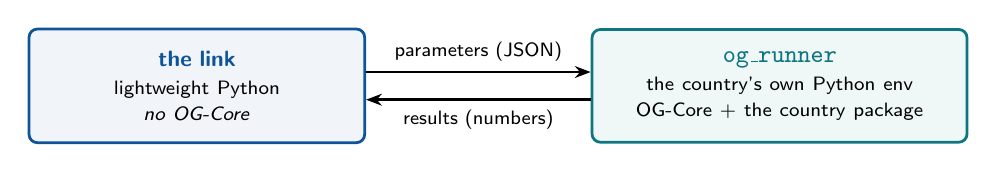
\begin{tikzpicture}[font=\footnotesize, every node/.style={align=center}]
    \node[draw=ogc, line width=1pt, rounded corners=3pt, fill=ogc!6, text width=3.7cm, inner sep=8pt] (link) at (0,0)
      {\textbf{\color{ogc}the link}\\[2pt]{\scriptsize lightweight Python\\ \emph{no OG-Core}}};
    \node[draw=clews, line width=1pt, rounded corners=3pt, fill=clews!6, text width=4.2cm, inner sep=8pt] (og) at (7.4,0)
      {\textbf{\color{clews}\code{og\_runner}}\\[2pt]{\scriptsize the country's own Python env\\ OG-Core + the country package}};
    \draw[-{Stealth[length=2mm]}, line width=1pt] ([yshift=5pt]link.east) -- node[above,font=\scriptsize]{parameters (JSON)} ([yshift=5pt]og.west);
    \draw[-{Stealth[length=2mm]}, line width=1pt] ([yshift=-5pt]og.west) -- node[below,font=\scriptsize]{results (numbers)} ([yshift=-5pt]link.east);
  \end{tikzpicture}
  \par\medskip
  \begin{itemize}\setlength\itemsep{6pt}\small
    \item The link has \textbf{no OG-Core inside it}; to solve, it launches the model in its own Python
          environment (found in a small registry).
    \item Only \textbf{data} crosses the line --- the changed parameters go in, the solved economy comes
          back as numbers (\code{serde.py}); no live objects are shared.
    \item The unchanged \textbf{baseline} is solved once and reused by every reform.
  \end{itemize}
\end{frame}

\begin{frame}{One run, end to end}
  Staged, and solved \textbf{once}:
  \medskip
  \begin{enumerate}\setlength\itemsep{5pt}\small
    \item \textbf{Export the baseline} (cached) and discover the energy ports (the concordance).
    \item \textbf{Pre-solve channels} (CLEWS$\to$OG) mutate the reform parameters.
    \item \textbf{Solve the reform} --- one subprocess solve.
    \item \textbf{Post-solve channels} (OG$\to$CLEWS) emit demand, the discount rate, the carbon penalty.
    \item \textbf{Report} --- macro table, incidence by income group, a provenance manifest.
  \end{enumerate}
  \vfill
  {\footnotesize\color{sub}\textbf{Country-agnostic}: onboard a country with \code{models register} (which
  discovers its calibration) plus a \code{CountryConfig}; the energy industry and good indices are discovered
  per run, and energy channels skip cleanly when electricity can't be isolated.}
\end{frame}

% ============================ 6. MUIOGO =================================
\sectiondiv{Use in MUIOGO}{From a CLEWS run to the economy, and back}

\begin{frame}{Reading a CLEWS run --- today}
  \begin{itemize}\setlength\itemsep{7pt}\small
    \item MUIOGO stores a solved CLEWS case under \code{DataStorage/.../res/.../csv/}.
    \item The link reads it directly: \code{muiogo\_run.py} locates the CSVs and
          \code{signals.commodity\_shadow\_price} reads the \textbf{commodity-balance dual} --- the
          marginal electricity price --- verified against a live MUIOGO run.
    \item That price (with emissions) drives a single \textbf{CLEWS$\to$OG pass}: channels $\to$ solve $\to$
          results (macro, incidence, health).
  \end{itemize}
  \vfill
  {\footnotesize\color{sub}This pass is validated end to end --- the
  energy\,$\to$\,investment\,$\to$\,carbon\,$\to$\,health suite converges.}
\end{frame}

\begin{frame}{Closing the loop into MUIOGO --- next}
  The OG$\to$CLEWS channels already produce the feedback artifacts --- \textbf{Demand},
  \textbf{DiscountRate}, \textbf{EmissionsPenalty} --- written as CSV patches (\code{clews\_io.py}).
  \medskip
  Three pieces remain to close the loop:
  \begin{enumerate}\setlength\itemsep{5pt}\small
    \item a MUIOGO \textbf{post-run hook} that calls the link after a CLEWS solve;
    \item a \code{clews\_runner} that feeds the patches through MUIOGO's endpoints
          (\code{updateData} $\to$ \code{createCaseRun} $\to$ \code{run}) and re-solves CLEWS;
    \item the \textbf{iterate} driver: re-solve, re-read the price, and repeat --- easing in each step so
          it settles --- until supply and demand agree.
  \end{enumerate}
  \vfill
  {\footnotesize\color{sub}Honest status: the demand channel is inert in a single pass (it says so in its
  own provenance); the single CLEWS$\to$OG pass runs today --- the round-trip is the next architectural piece.}
\end{frame}

% ============================ CLOSE ====================================
\begin{frame}{What the coupling adds}
  Neither model alone produces this:
  \medskip
  \begin{itemize}\setlength\itemsep{7pt}
    \item \textbf{Who} an energy-system change helps or hurts --- the effect by age and income group.
    \item \textbf{What cleaner air is worth} --- in lives, and in a more productive workforce.
    \item A \textbf{mutually consistent} energy--economy outcome, rather than each side assuming the other.
  \end{itemize}
  \vfill
  {\footnotesize\color{mute}\texttt{ogclews-link}\, $\cdot$\, OG-PHL calibration\, $\cdot$\, figures in
  \texttt{presentation/coupling-diagrams/}}
\end{frame}

\end{document}
